\documentclass[
    ebook,
    11pt,
    twoside,
    onecolumn,
    openright,
    final
    % draft
]{memoir}

\usepackage[]{geometry}
% \usepackage[final]{microtype}

\usepackage{amsmath}
\usepackage{amsfonts}
\usepackage{amssymb}

\usepackage{graphicx}

\usepackage{natbib}

\usepackage{kotex}
\usepackage{lipsum}

\usepackage{hyperref}
\hypersetup{%
    unicode=true,
    colorlinks=false
}

\usepackage{xcolor}

\begin{document}

\begin{titlingpage}
    \title{\HUGE\textbf{Notes on Electrodynamics}}
    \author{\Large\textbf{Nanaki}}
    \date{\Large{\today}}

    \pagenumbering{Alph}
    \maketitle
    \begin{center}
        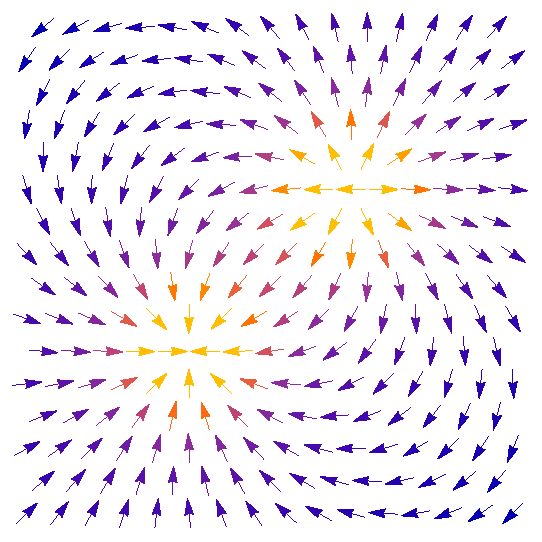
\includegraphics[width=0.8\textwidth]{figures/cover.pdf}
    \end{center}
\end{titlingpage}

\frontmatter

\tableofcontents
% \clearpage

\mainmatter

% === Introduction ===
\part{Introduction}
\chapter{Classical Electrodynamics and Special Relativity}


% === Special Relativiy ===
\part{The Special Theory of Relativity}

\chapter{The Principle of Relativity}
\section{Velocity of Propagation of Interaction}


\chapter{Physical Interpretation}

\chapter{Minkowski Geometry}

\chapter{Relativistic Mechanics}

% === Classical Electrodynamics ===
\part{Foundation of Electrodynamics}

\chapter{Charges in Electromagnetic Fields}

\chapter{The Electromagnetic Field Equations}

\chapter{Constant Electromagnetic Fields}

% === Electrodynamics of Continuous Media
\part{Electrodynamics of Continuous Media}

\chapter{Electrostatics of Conductors}

\chapter{Electrostatics of Dielectrics}

\chapter{Steady Current}

\chapter{Magnetostatics}

\chapter{Ferromagnetism and Antiferromagnetism}

\chapter{Quasi-Static Electromagnetic Field}

% === Electromagnetic Waves ===
\part{Electromagnetic Waves}

\chapter{Electromagnetic Waves}

\chapter{The Propagation of Electromagnetic Waves}

\chapter{The Field of Moving Charges}
% 2-VIII 8-XIV

\chapter{Radiation of Electromagnetic Waves}

\chapter{Scattering of Electromagnetic Waves}

\chapter{Diffraction of Electromagnetic Waves}
% 2-59 2-60 2-61

% === Appendices ===
\appendix
\part{Appendix}

\chapter{Mathematical Tools}
% Multipole Expansion

\backmatter

\end{document}
